\documentclass[11pt,a4paper,twoside]{article}
%
\usepackage[T1]{fontenc}
\usepackage[utf8]{inputenc}
\usepackage[francais]{babel}
\selectlanguage{francais}
\usepackage{url}
\usepackage{graphicx}
\usepackage{subfig}
\usepackage{float}

% Separateur milliers
\usepackage{siunitx}

%

% ---- MISE EN PAGE ----
\setlength{\parindent}{0em}
\setlength{\parskip}{0.6em}

% ----- CODE ----
\usepackage{color}

\definecolor{pblue}{rgb}{0.13,0.13,1}
\definecolor{pgreen}{rgb}{0,0.5,0}
\definecolor{pred}{rgb}{0.9,0,0}
\definecolor{pgrey}{rgb}{0.46,0.45,0.48}
\definecolor{light-gray}{gray}{0.95}

\usepackage{listings}
\lstset{language=Java,
  showspaces=false,
  showtabs=false,
  breaklines=true,
  showstringspaces=false,
  breakatwhitespace=true,
  commentstyle=\color{pgreen},
  keywordstyle=\color{pblue},
  stringstyle=\color{pred},
  basicstyle=\fontsize{11}{11}\ttfamily,
  backgroundcolor=\color{light-gray},
  numbers=left
}

% ---- EN-TETE ET TITRE ----
\usepackage[hcentering=true,nomarginpar,textwidth=426.8pt,textheight=650.2pt,headheight=24pt]{geometry}
\geometry{bmargin=1.5cm, tmargin=1.5cm}
\usepackage{fancyhdr}
\fancypagestyle{plain}{
\fancyhf{}
\renewcommand{\headrulewidth}{0pt}
\renewcommand{\footrulewidth}{0pt}}
\pagestyle{fancy}
\fancyhf{}
\fancyhead[LO]{MCR --- Printemps 2017}
\fancyhead[RO,LE]{\thepage}
\fancyhead[RE]{Clavien, Gonzalez Montes, Milani, Guillod, Luthier}
\renewcommand{\headrulewidth}{0.4pt}
\renewcommand{\footrulewidth}{0pt}



  \title{\huge\bfseries Modèle de conception Visiteur}
  \author{Tony \bsc{Clavien}, Nathan \bsc{Gonzalez Montes}, \\ Guillaume \bsc{Milani}, Maxime \bsc{Guillod}, Gabriel \bsc{Luthier}}
  \date{\today}

% Compteur de sections
\renewcommand{\thesubsection}{\arabic{subsection})}
\newcommand{\p}{0,374}

%%%
\begin{document}
\maketitle
%
\section*{Introduction}
Ce projet a été réalisé dans le cours de Modèles de Conception Réutilisables (MCR) de la HEIG-VD au semestre de printemps 2017. Il a pour but de montrer un exemple du modèle de conception \texttt{Visiteur} dans le cadre d'une application ludique.

Nous avons réalisé un jeu mettant en scène les personnages du film \og Les Visiteurs \fg.

\section*{Règles du jeu}
Le jeu se joue à deux joueurs, sur le même clavier. Chaque visiteur peut se déplacer à gauche ou à droite (Touches A et D pour Jacquouille et flèches gauche ou droite pour Hubert de Montmiraille) et essaie d'intercepter des objets qui tombent du ciel.

Chaque objet intercepté a un effet sur les points de vie et le score du joueur qui l'intercepte. La figure \ref{regles} est affichée au lancement du jeu et décrit l'effet de chaque objet sur chaque joueur.
\begin{figure}[!ht]
	\center
	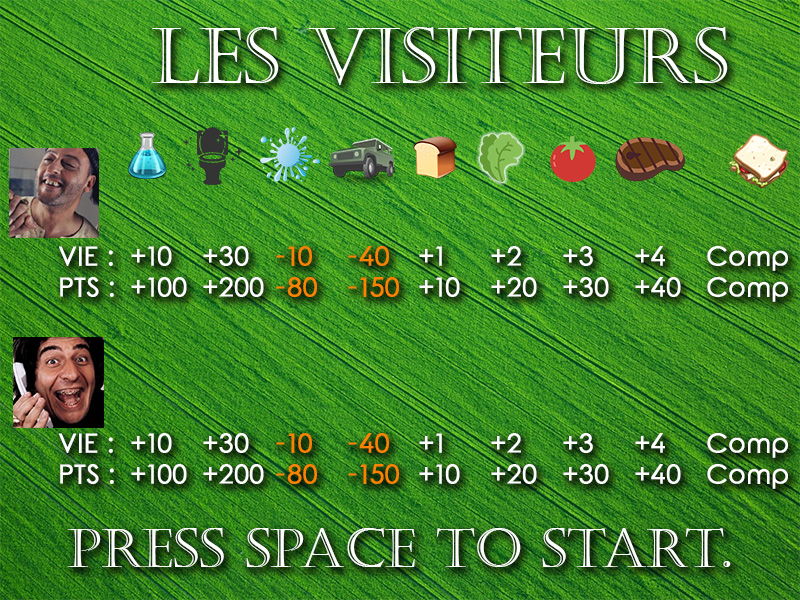
\includegraphics[scale=0.5]{../Game/src/resources/images/regles}
	\caption{Règles du jeu}
	\label{regles}
\end{figure}

\begin{figure}[!ht]
	\center
	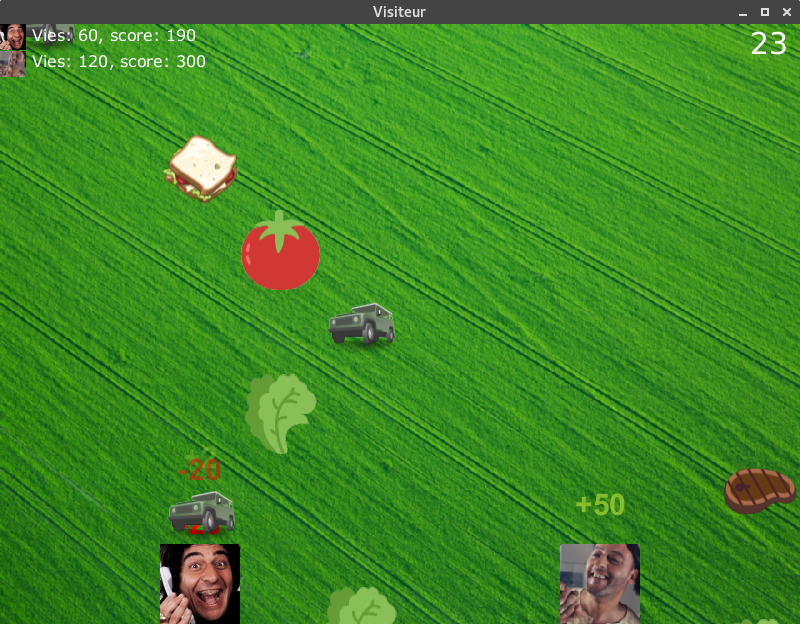
\includegraphics[scale=0.5]{capture_jeu.png}
	\caption{Exemple d'une partie}
	\label{partie}
\end{figure}
\newpage

\section*{Implémentation}
Les deux joueurs implémentent l'interface \texttt{Visiteur} et de ce fait une méthode \texttt{visite} pour chaque type d'obstacle. Quand il y a collision entre un joueur et un objet, le joueur \og visite \fg l'objet afin de définir son type et perd ou gagne le nombre de point voulu. Cette implémentation permet de manipuler dans la classe principale \texttt{Game} que des \texttt{Joueur} et \texttt{Obstacle}, sans savoir de quel type d'\texttt{Obstacle} (puisque c'est le joueur qui le détermine en le visitant).

L'utilisation du modèle \texttt{Visiteur} permet d'ajouter les actions des objets (i.e. enlever / donner des vies ou des points de score) sans modifier le code de ces derniers. Les objets (\texttt{Toilette}, \texttt{Flaque}, \texttt{Voiture} etc.) pourraient être utilisés à l'extérieur de cette application sans que leur rôle dans le jeu n'apparaisse (puisqu'ils n'ont de particulier qu'une méthode \texttt{accepte(Visiteur v)}).

Finalement, certains obstacles sont composés d'autres obstacles (\texttt{Sandwich} par exemple). L'utilisation de ce modèle de conception permet que les joueurs ignorent la nature exacte de l'obstacle (il ne sait pas qu'il s'agit d'une composition), il visite de la même manière chaque obstacle et c'est l'obstacle lui-même qui appelle la méthode \texttt{accepte(Visiteur v)} des éléments qui le composent.

\section*{Diagramme UML}
Le diagramme UML est annexé à ce document en raison de sa grande taille.

\end{document}
